% ПЛАН
%# Глава 3 – Численные методы для нахождение оптимальной несмещенной оценки параметров гармоник
%
%Выводы по главе:
%
%- Методы, основанные на интерполировании смежных гармоник, позволяют достичь высокой точности, во многих случаях достаточной для практического применения, однако они не позволяют достичь точности оптимальной несмещенной оценки.
%- Можно выделить два подхода к построению алгоритмов на основе корреляционного анализа: использование итерационного процесса для нахождения частоты, амплитуды и фазы каждой гармоники и использование техники дополнения нулями сигнала с целью уплотнения гармоник в спектре сигнала. Оба метода требуют существенно больших вычислительных ресурсов, чем методы основанные на интерполировании, но обеспечивают оптимальную несмещенную оценку.
%- Время расчета параметров гармоник многотонального сигнала с помощью техники дополнения нулями может быть существенно снижено за счет применения разряженного быстрого преобразования Фурье.
%- Реализация итерационного оптимизационного метода нахождения гармоник на основе чисел Фиббоначи при небольшом числе обсчитываемых гармоник обеспечивает быстродействие, близкое к итерационным методам. 
%- Реализация метода дополнение нулями сигнала при использовании разряженного преобразования Фурье имеет быстродействие менее чем на порядок худшее, чем итерационные методы, при этом быстродействие не зависит от числа обсчитываемых гармоник. Также нужно отметить больший объем памяти, требуемый для этого метода, который при этом не является критичным для современных вычислительных устройств.
%


\chapter{Численные методы для нахождения оптимальной несмещенной оценки параметров гармоник}\label{ch:ch3}

\section{Применение быстрых алгоритмов для выполнения фильтрации изображений} \label{sec:ch3/sect1}
% Васеева Т. В., Альтман Е. А., Малютин А. Г. ПРИМЕНЕНИЕ БЫСТРЫХ АЛГОРИТМОВ ДЛЯ ВЫПОЛНЕНИЯ ФИЛЬТРАЦИИ ИЗОБРАЖЕНИЙ //Современные проблемы радиоэлектроники. – 2018. – С. 162-165.

В современных технических устройствах широко применяются различные методы по получению, преобразованию, передаче и извлечению информации из различных изображений. Одной из основных операций в обработке изображений и сигналов является фильтрация \cite{gonzalez2018digital}. 
% 1. Gonzalez R.C., Woods R.E. Digital image processing. New York, NY, Pearson, 2007 (Russ. ed.: Gonsales R., Vuds R. Tsifrovaya obrabotka izobrazhenii. 3rd ed. Moscow, Tekhnosfera Publ., 2012. 1104 p.).
Фильтрация используется как для снижения уровня шумов в изображении, так и для выявления содержащейся в них полезной информации, а также при различных преобразованиях изображений.

Фильтром называют устройство, выполняющее фильтрацию. Эффект, который накладывает фильтр на изображение, зависит от его коэффициентов. Все виды фильтров можно разделить на классы: частотные линейные, нелинейные, комбинированные, гибридные и адаптивные. Линейные фильтры имеют простое математическое описание. Фильтрация производится с помощью дискретной свертки, в ходе обработки используется небольшой прямоугольный или квадратный участок, на котором определяется функция. Размер данного участка называют апертурой фильтра, а заданную функцию – весовой. Апертуру совместно с заданной функцией называют маской изображения или ядром фильтра \cite{bondina2012comparative}.
% 2. Бондина Н. Н., Калмычков А. С., Кривенцов В. Э. Сравнительный анализ алгоритмов фильтрации медицинских изображений //Вестник Национального технического университета Харьковский политехнический институт. Серия: Информатика и моделирование. – 2012. – №. 38.

В статье \cite{application_of_fast2018} рассматриваются быстрые алгоритмы для выполнения операции фильтрации изображений. Быстрые алгоритмы позволяют увеличить производительность работы фильтрации за счет использования меньшего числа операций для достижения конечного результата.

Выбор быстрого алгоритма фильтрации определяется прикладной задачей. Существуют несколько видов фильтров: шума, низких частот, морфологические, медианные, blur/sharp и другие. Рассмотрим некоторые из них.

Фундаментальной проблемой в области обработки изображений является удаление шума. Изображение – это двумерный или векторный сигнал, содержащий огромное количество информации. Цифровой шум – это мелкие детали на изображении (частицы), которые выглядят как светлые, темные или цветные точки. Причины зашумленных изображений различны: искажения, качество аппаратуры, неравномерная прозрач-
ность воздушного слоя, пыль и другие причины. Сложность решения данной проблемы зависит от характера шумов.

В цифровой обработке сигналов широко используются методы линейной фильтрации изображений (сглаживающие или усредняющие). В случае комбинированного шума можно применять линейные и нелинейные фильтры или использовать гибридные фильтры 
\cite{Soynikova2016high-performance}.
% 3. Сойникова Е. С. и др. Высокопроизводительный метод анализа и морфологической обработки изображений //Научный результат. Информационные технологии. – 2016. – Т. 1. – №. 3.

Применение медианных фильтров эффективно для некоторых видов шума и периодических помех без одновременного искажения сигнала. Медианные фильтры удобны для борьбы с импульсным (точечным) шумом. Медианные фильтры сохраняют контуры изображения. Основные недостатки медианных фильтров заключаются в подавлении гауссова шума и появлении размытых контуров деталей. Для устранения этих
недостатков используют метод ранговой статистики – рекурсивный ранжирующий фильтр. Для некоторых операций целесообразно использовать нелинейные фильтры, например, импульсный шум лучше удаляется нелинейным фильтром на основе ранговой статистики, при этом сохраняются перепады в изображении \cite{gruzman2002digital}.
% 5. Грузман И. С. и др. Цифровая обработка изображений в информационных системах //Новосибирск: изд-во НГТУ. – 2002. – Т. 352. – С. 6.

В статье \cite{7025588}рассмотрен высокопроизводительный метод анализа и морфологической обработки изображений. 
% 4. S. Yoshizawa and H. Yokota, "Fast L1 Gaussian convolution via domain splitting," 2014 IEEE International Conference on Image Processing (ICIP), Paris, France, 2014, pp. 2908-2912, doi: 10.1109/ICIP.2014.7025588.
Математическая морфология – инструмент для выделения и анализа на изображении графических элементов с известной геометрической структурой. Базовое описание термина было дано в теории множеств. Предполагается, что любой объект на изображении можно представить в виде множества в двумерном пространстве. Морфологические методы применяются в основном для работы с двоичными (черно-белыми) изображениями. Входными данными для аппарата математической морфологии являются два изображения (обрабатываемое и специальное). Специальное изображение называют примитивом (primitive) или структурным элементом (structure elements). Структурный элемент описывает область с некоторой формой, которую можно представить в виде бинарного изображения заданного размера. Результаты метода морфологической обработки зависят от размера структурного элемента ($3\times3$, $4\times4$, $5\times5$ пикселов) и конфигурации исходного элемента. Основные операции математической морфологии:

\begin{enumerate}
\item дилатация или расширение (dilation), увеличивает область изображения, устраняет разрывы линий на изображении путем их перекрытия;

\item эрозия (erosion), уменьшает область изображения, исключает из изображения несуществующие по размеру детали;

\item размыкание (opening), помогает избавиться от маленьких фрагментов, которые выступают наружу области за ее границы;

\item замыкание (closing), позволяет сомкнуть внутреннее отверстие области и устранить заливы вдоль границы области.
\end{enumerate}

Обработка изображения методом blur/sharp (размытие/резкость) делает его контрастнее и приятнее для восприятия. Основной принцип метода заключается в том, что фильтр Gaussian blur размывает поверхность и сглаживает неровности краев изображения. Фильтр Unsharp mask позволяет выделить границы, края и линии на объекте. Алгоритм Sharp позволяет восстановить мелкие детали изображения, если детали были потеряны из-за естественного размытия изображения с объектива камеры или качество
изображения низкое. При наложении размытого слоя на слой повышенной четкости, происходит размытие поверхности, уменьшение дефектов на поверхности изображения. Одновременно увеличивается резкость в гранях, углах и линиях.

Из всего разнообразия цифровых фильтров существенно сократить количество операций без изменения конечного результата можно лишь для линейных фильтров, в которых используется математическая операция двумерной свертки \cite{bluehut1989fast}. 
% 6. Блейхут Р. Э. Быстрые алгоритмы цифровой обработки сигналов. – Мир, 1989.
Классификация методов быстрых вычислений двумерных корреляций и сверток приведена ниже \ref{img:picture3.1}.

При цифровой обработке сигналов часто применяют две схожие операции: свертка (convolution) и корреляция (correlation). 

Для уменьшения количества вычислительных операций для задач фильтрации изображения (двумерной свертки) рассмотрим три варианта вычисления:

\begin{enumerate}
	\item вычисление по формуле двумерной свертки;
	 
	\item использование двумерных сверток меньших размеров \cite{550562};
	
	\item использование быстрых алгоритмов одномерной свертки для вычисления двумерной свертки \cite{MOU1987377}. 
\end{enumerate}
% 7. Y. Naito, T. Miyazaki and I. Kuroda, "A fast full-search motion estimation method for programmable processors with a multiply-accumulator," 1996 IEEE International Conference on Acoustics, Speech, and Signal Processing Conference Proceedings, Atlanta, GA, USA, 1996, pp. 3221-3224 vol. 6, doi: 10.1109/ICASSP.1996.550562.

% 8. Mou Z. J., Duhamel P. Fast FIR filtering: algorithms and implementations //Signal Processing. – 1987. – Т. 13. – №. 4. – С. 377-384.
\begin{figure}[ht]
	\centering
	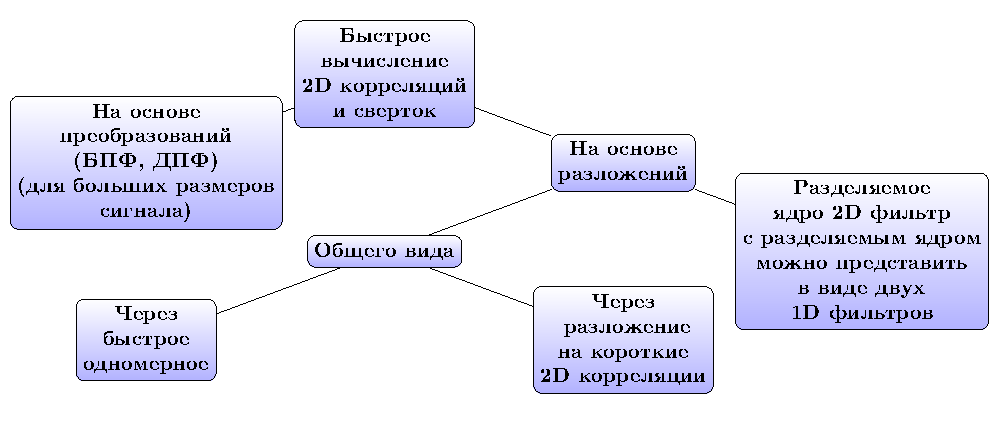
\includegraphics [scale=0.9] {Classification_of_methods_for_fast computation_of_two-dimensional correlations_and_convolutions.pdf}
	\caption{Классификация методов быстрых вычислений двумерных корреляций и сверток.}
	\label{img:picture3.1}
\end{figure}

Сразу отметим, что наиболее известный способ быстрого вычисления корреляции с использованием быстрого преобразования Фурье плохо подходит для рассматриваемой задачи. При использовании БПФ для вычисления свертки или корреляции требуется предварительное выполнение дополнительных операций, переводящих вычисление свертки или корреляции в частотную область. При больших размерах обрабатываемых сигналов эти дополнительные расходы незначительны, однако, даже если один из сигналов имеет малое число отсчетов (единицы или десятки), дополнительные расходы делают весь метод неэффективным \cite{altman2015fast}. В нашем случае, апертура цифрового фильтра для всех рассмотренных выше примеров будет небольшой.
% Альтман Е. А., Захаренко Е. И. Быстрый алгоритм вычисления двумерной корреляции для видеообработки //Доклады Томского государственного университета систем управления и радиоэлектроники. – 2015. – №. 2 (36).

Анализируя приведенные выше примеры цифровых фильтров нужно отметить,
что часть из них использует так называемое разделимое ядро. Разделимое ядро цифрового фильтра позволяет разделить операцию двумерной свертки на две последовательно выполняемые операции одномерной свертки. Очевидно, такое преобразование операции фильтрации позволяет значительно сократить число требуемых арифметических операций. Разделимое ядро является самым эффективным способом построения быстрого алгоритма вычисления свертки, поэтому разработчики фильтров стремятся использовать именно такие ядра.

После разделения к полученным одномерным фильтрам могут быть применены методы снижения числа операций, используемые для одномерных фильтров сигналов. Хотя, с учетом малой длины фильтра, выигрыш в этом случае не так велик, как при разделении ядра. В то же время немалое число полезных фильтров для изображений используют ядра общего вида, поэтому задача построения быстрых алгоритмов для двумерных сверток вида остается весьма актуальной.

В работе \cite{altman2015fast} приведен обзор быстрых алгоритмов для вычисления коротких двумерных корреляций. Учитывая полную аналогию между операциями свертки и корреляции, мы можем перенести полученные в этой статье результаты на быстрые алгоритмы для коротких двумерных сверток. Можно сделать вывод, что быстрые алгоритмы коротких сверток позволяют улучшить быстродействие операции фильтрации изображения на десятки процентов. Такой выигрыш хотя и не позволяет вывести методы обработки изображений на качественно новый уровень, но вместе с тем значимо улучшает параметры устройств, использующих эти алгоритмы. В некоторых случаях при реализации фильтров с разделимым ядром количество требуемых операций может быть сокращено в несколько раз. 

Например, как показано в \cite{altman2015fast}, быстрые алгоритмы вычисления двумерной свертки
имеет смысл применять, начиная с размера ядра, равного $4\times4$. Практически применяются ядра нечетных размеров. Сокращение числа требуемых операций при применении разложения при ядре $5\times5$ составляет $16\%$, $7 \times 7 $ - 27\%, $9 \times 9$ - 3\%. Ввиду сложности
алгоритма разложения на свертки меньших размеров при практической реализации следует ожидать уменьшение выигрыша в быстродействии. Тем не менее следует сделать вывод, что быстрые алгоритмы вычисления двумерной свертки имеют практическую ценность для вычисления коротких сверток для ядер, начиная с размера $5\times5$.

Использование общих подходов к построению быстрых алгоритмов в целом применимо для построения быстрых фильтров изображений. Вместе с тем при выборе алгоритмов и их параметров для программной или аппаратной реализации требуется учитывать особенности двумерных фильтров изображений, прежде всего, небольшой размер ядра.

\section{Интерполяционные методы} \label{sec:ch3/sect2}
Для интерполяционных методов существует единый алгоритм оценки амплитуды и фазы гармонических составляющих напряжения. Базовым элементом для нахождения амплитуд и фаз гармонических составляющих напряжения является параметр $\delta$ \cite{558515}. 
% 109. B. G. Quinn, "Estimation of frequency, amplitude, and phase from the DFT of a time series," in IEEE Transactions on Signal Processing, vol. 45, no. 3, pp. 814-817, March 1997, doi: 10.1109/78.558515.

Если параметр $\delta$ известен, то амплитуда гармоник напряжения определяется из следующего выражения \cite{558515}:

\begin{equation}
	\label{eq:equation3.11}
	A = T^{-1} \cdot \frac{\left|{\displaystyle\sum_{t=-1}^{1} y(k+t)\overline{c_t}} \right| }{\displaystyle\sum_{k=-1}^{1}|c_t|^2}
\end{equation}

где $T$ – период напряжения;

$\overline{c_t}$ – среднеарифметическое значение $c_t$;

$c_t$ – определяется из выражения:

\begin{equation}
	\label{eq:equation3.12}
	c_t = \frac{[e^{2 \cdot \pi \cdot j \cdot \delta} - 1]}{[4 \cdot \pi \cdot j \cdot (\delta - t)]}
\end{equation}

Фаза  $\nu$-й гармоники напряжения вычисляется по следующей формуле:

\begin{equation}
	\label{eq:equation3.13}
	\varphi_\nu = \mathrm{arg} \left({\displaystyle\sum_{t=-1}^{1} y(k+t) \cdot \overline{c_t} }\right)
\end{equation}

Листинг программы, реализующий алгоритм оценки амплитуды и фазы гармоник напряжения для интерполяционных методов приведен в \textbf{приложении ?}.

\section{Метод корреляционных функций} \label{sec:ch3/sect3}

Корреляционный анализ широко применим для решения технических задач \cite{Oppenheim2018Digital}. 
% Оппенгейм А., Шафер Р. Цифровая обработка сигналов. – Litres, 2018.
В работах \cite{Elizarov2012application, Altman2012improvement} описаны практические реализации подходов для решения задач оценки гармонических составляющих напряжения. 
%Елизаров Д. А. Применение метода чисел Фибоначчи для поиска максимума корреляционной функции //В мире научных открытий. – 2012. – №. 1. – С. 28-38.

% Альтман Е. А., Елизаров Д. А., Чижма С. Н. Совершенствование алгоритма определения параметров гармоник сигналов в электрической сети для оценки качества электроэнергии //Электротехнические комплексы и системы управления. – 2012. – №. 4. – С. 5-9.

Базовым параметром метода корреляционных функций является коэффициент корреляции. Для исследуемой функции напряжения формируется набор эталонов. Далее производится анализ на наличие связи в точках между параметрами исследуемого напряжения и эталона. Наибольшее значение коэффициента корреляции показывает на эталон, параметр которого необходимо выбрать. 

Для того чтобы сформировать набор эталонов необходимо определить базовую точку, вокруг которой будут создаваться эталоны (обозначим ее через $B$). Эта точка выбирается из ближайших целых значений основной частоты измеряемого напряжения. Также необходимо определить шаг, с которым будут формироваться эталоны (обозначим его через $h$ ). Затем на промежутке [$B - \sfrac{1}{2}$, $B + \sfrac{1}{2}$]   необходимо произвести формирование эталонов. Для этого спектр оконной функции необходимо сдвигать вправо и влево с шагом в пределе заданного промежутка и определять $5$ точек вокруг пика. 

Расчет коэффициента корреляции производиться по $5$ точкам, так как для дискретного спектра энергия гармоники (порядка $80$ \%) сосредоточена в ближайших $3-5$ отсчетах в районе максимума амплитудного спектра. Возможность смещать спектр на заданную величину без изменения амплитудного спектра обеспечивается свойством ДПФ \cite{sergienko2011digital}.
%Сергиенко А. Б. Цифровая обработка сигналов. – БХВ-Петербург, 2011.
Согласно данному свойству необходимо спектр окна домножить на величину $e^{-j \cdot \frac{2 \cdot \pi (B \pm i \cdot h)}{T_w}}$

Таким образом, получается набор эталонных множеств из $М$  точек $W_j = {W_{j0}, W_{j1}, \cdots, W_{jM-1} }$ , каждая точка которого вычисляется по правилу:

\begin{equation}
	\label{eq:equation3.1}
W_{ji} = W \left( {\frac{2 \cdot \pi}{T_w} \cdot (i + \bigtriangleup r_j)}\right) 
\end{equation}

где $- \frac{M}{2} < i < \frac{M}{2}$, $0 < \bigtriangleup r_j < 1$

На рисунке \textbf{?} показан пример построения наборов эталонов (здесь представлено три набора). Первый набор не имеет смещения относительно базовой точки. Второй набор смещен влево относительно базовой точки на величину шага формирования эталона $h$  . Третий набор смещен вправо относительно базовой точки B на величину шага формирования эталона $h$. Также для первого набора эталона определены его отсчеты БПФ. 

Пусть имеется напряжение $u'(t)$ с периодом $T_s$ и спектром, ограниченным  $N$-ой гармоникой, и белым шумом $\eta$. Для ограничения длительности напряжения накладывается некоторое окно $w(t)$, имеющее отличное от нуля значение на временном отрезке $[- \frac{T_w}{T_w}, - \frac{T_w}{T_w}] $ и спектром $W(\omega)$. 

В качестве весовой функции для метода корреляционных функций применяется окно Кайзера с параметром $10$. Окно Кайзера на 2048 точек с параметром $10$ представлено на рисунке \textbf{?}. Основные свойства весовой функции Кайзера, а также формула для определения коэффициентов приведены в таблице \ref{app:А}.

\begin{equation}
	\label{eq:equation3.2}
	u(t) = u'(t) \cdot w(t) = \displaystyle\sum_{\nu=0}^{\nu=N} A_\nu e^{j \cdot \varphi_\nu} w(t) e^{j \cdot \frac{2 \cdot \pi}{T_s} \cdot \nu \cdot t} + \eta (t) \cdot w(t) = \displaystyle\sum_{\nu=0}^{\nu=N} A_\nu e^{j \cdot \varphi_\nu} w(t) \cdot e^{j \cdot \frac{2 \cdot \pi}{T_s} \cdot \nu \cdot t} +\eta_w(t)
\end{equation}

Спектр сигнала $w(t) \cdot e^{j \cdot \frac{2 \cdot \pi}{T_s} \cdot \nu \cdot t}$, как известно из свойств преобразования Фурье, представляет собой смещенный на величину $\frac{2 \pi}{T_s} \cdot \nu$ спектр сигнала $w(t)$, a именно $W \left( {\omega - \frac{2 \cdot \pi}{T_s} \cdot \nu} \right)$.


Спектр сигнала $\eta_w(t)$ есть произведение во временной области функции $\eta(t)$ и $w(t)$, то в частотной области спектр этого сигнала есть свертка спектров указанных функций \cite{Increase_Accuracy_Yelizarov2014}:

\begin{equation}
	\label{eq:equation3.3}
	\Theta_w(\omega) = \int\limits_{- \infty}^{\infty} \Theta (\Omega) W(\omega - \Omega) \mathrm{d}\Omega
\end{equation}

Величина $\Theta_w(\omega)$, как и $\Theta(\omega)$, является случайной. Исходя из \cite{Increase_Accuracy_Yelizarov2014} дисперсия   не зависит от частоты   и равна \cite{Altman2012formation, Davenport1960introduction}:

% 36. Давенпорт В. Б., Рут В. Л. Введение в теорию случайных сигналов и шумов. М.: ИЛ. – 1960.

% 84. Альтман Е. А., Елизаров Д. А. Формирование эталонной функции с действительным спектром для оценки спектра сигнала электрической сети //Динамика систем, механизмов и машин. – 2012. – №. 1.

\begin{equation}
	\label{eq:equation3.4}
	D[\Theta_w(\omega)] = D[\Theta(\omega)] \cdot \frac{1}{T_w} \cdot \int\limits_{- \sfrac{T_w}{2}}^{\sfrac{T_w}{2}} w^2 (t) \mathrm{d}t = const  
\end{equation}

Следовательно, спектр напряжения $u(t)$  представляет собой взвешенную сумму спектров наложенного окна $W\left( {\omega - \frac{2 \cdot \pi}{T_s} \cdot \nu}\right)$   и случайной величины $\Theta_w(\omega)$  
\cite{Increase_Accuracy_Yelizarov2014}:

\begin{equation}
	\label{eq:equation3.5}
	U(\omega) = \displaystyle\sum_{\nu=0}^{\nu=N} A_{\nu} e^{j \cdot \varphi_\nu} W\left( {\omega - \frac{2 \cdot \pi}{T_s} \cdot \nu}\right) + \Theta_w(\omega)  
\end{equation}

Задача измерения гармонических составляющих напряжения $u'(t)$, ограниченных во временной области окном $w(t)$ сводится к нахождению коэффициента $A_\nu$ по $M$ точкам функции $U(\omega)$ в области $v$-го пика. Шум $\Theta_w(\omega) $   определяет максимальную точность вычисления параметра гармонических составляющих напряжения в соответствии с теоретической границей Крамера-Рао. Нижняя граница Крамера-Рао является объективным показателем для определения границы дисперсии ошибки при оценке неизвестного параметра при использовании различных методов. 

Найдем значение функции $U(\omega)$  в этих точках. Так как эти точки получаются при помощи вычисления БПФ дискретизированного сигнала на временном отрезке $T_w$ (ширина окна), то в результате применения этого алгоритма мы получаем значение спектра в равномерно отстоящих точках $ \omega = \frac{2 \cdot \pi}{T_w} \cdot n$. После подстановки   в \ref{eq:equation3.5} выражение в районе пика БПФ $\nu$ имеет вид:

\begin{equation}
	\label{eq:equation3.6}
	U \left(\frac{2 \cdot \pi}{T_w} \cdot n \right) = \displaystyle\sum_{\nu=0}^{\nu=N} A_{\nu} e^{j \cdot \varphi_\nu} W\left( {\frac{2 \cdot \pi}{T_w} \cdot n - \frac{2 \cdot \pi}{T_s} \cdot \nu }\right) = \displaystyle\sum_{\nu=0}^{\nu=N} A_{\nu} e^{j \cdot \varphi_\nu} W \left({\frac{2 \cdot \pi}{T_w} \cdot \left( {n - \frac{T_w}{T_s} \cdot \nu} \right) } \right) + \Theta_w(\omega)
\end{equation}

Пусть целая часть выражения в \ref{eq:equation3.6} $ n - \frac{T_w}{T_s} \cdot \nu$  равна $r$ , а дробная часть этого выражения равна $ \bigtriangleup r$ . Тогда: 

\begin{equation}
	\label{eq:equation3.7}
	U \left(\frac{2 \cdot \pi}{T_w} \cdot n \right) = \displaystyle\sum_{\nu=0}^{\nu=N} A_{\nu} e^{j \cdot \varphi_\nu} W\left( {\frac{2 \cdot \pi}{T_w} \cdot (r + \bigtriangleup r ) }\right) + \Theta_w(\omega)
\end{equation}

Таким образом, получается реализация БПФ напряжения ограниченного окном, для которой: $U = {U_0, U_1, \cdots , U_M} $ – множество из $M$ точек этого БПФ в области пика $\nu$.
Коэффициент корреляции между множеством $U$ и эталоном $W_j$ определяется по формуле:

\begin{equation}
	\label{eq:equation3.8}
	\displaystyle\sum_{i=1}^{i=M} U_i W_{ji} = \displaystyle\sum_{i=1}^{i=M} A_{\nu} e^{j \cdot \varphi_\nu} W\left( {\frac{2 \cdot \pi}{T_w} \cdot (i + \bigtriangleup r ) }\right) \cdot W\left( {\frac{2 \cdot \pi}{T_w} \cdot (i + \bigtriangleup r_j ) }\right) = A_{\nu} e^{j \cdot \varphi_\nu} R (\bigtriangleup r - \bigtriangleup r_j) \Theta_w(\omega)
\end{equation}

где $R (\bigtriangleup r - \bigtriangleup r_j)$ – корреляционная функция $W\left( {\frac{2 \cdot \pi}{T_w} \cdot (i + \bigtriangleup r) }\right)$  и $W\left( {\frac{2 \cdot \pi}{T_w} \cdot (i + \bigtriangleup r_j) }\right)$. 

При определении гармонических составляющих напряжения будет достаточно рассматривать $5$ гармоник возле максимальной гармоники спектра напряжения, т.~е. $M = 5$ \cite{Increase_Accuracy_Yelizarov2014}.
 
Если в качестве окна выбирается симметричная функция, то функция $W(\omega)$  и множество ее значений $W_ji$  будут действительными. С учетом этого, модуль амплитуды  $\nu$-й гармоники определяется следующим образом \cite{Increase_Accuracy_Yelizarov2014}:

\begin{equation}
	\label{eq:equation3.9}
	A_{\nu} = \frac{1}{R(\bigtriangleup r - \bigtriangleup r_j)} \cdot \sqrt{\left({\displaystyle\sum_{i=1}^{i=M}\mathrm{Re}(U_i) \cdot W_{ji}} \right)^2 + \left({\displaystyle\sum_{i=1}^{i=M}\mathrm{Im}(U_i) \cdot W_{ji}} \right)^2 - \frac{\Theta_w(\omega)}{R(\bigtriangleup r - \bigtriangleup r_j)}}
\end{equation}

Для случая, когда эталоны $W_{ji}$ формируются достаточно часто, корреляционную функцию $R(\bigtriangleup r - \bigtriangleup r_j) $  можно считать равной $1$, тогда параметр шума $\Theta_w(\omega)$ не учитывается, а считается теоретической погрешностью метода \cite{Increase_Accuracy_Yelizarov2014}. Тогда формулу для модуля амплитуды  $\nu$-й гармоники \ref{eq:equation3.9} можно переписать следующим образом:

\begin{equation}
	\label{eq:equation3.10}
	A_{\nu} =  \sqrt{\left({\displaystyle\sum_{i=1}^{i=M}\mathrm{Re}(U_i) \cdot W_{ji}} \right)^2 + \left({\displaystyle\sum_{i=1}^{i=M}\mathrm{Im}(U_i) \cdot W_{ji}} \right)^2}
\end{equation}

Соответственно, необходимо из набора  эталонов $W_ji$ выбрать тот, который наиболее точно соответствует множеству $U$. В качестве критерия точности соответствия выберем минимум выражения $ \left|{\bigtriangleup r - \bigtriangleup r_j}\right| $. Очевидно, что чем меньше значение этого выражения, тем больше значение корреляционной функции $R(\bigtriangleup r - \bigtriangleup r_j)$ и вычисляемого модуля гармоники $A_\nu$ \cite{Increase_Accuracy_Yelizarov2014}. 

Наибольшее значение модуля амплитуды гармоники показывает на пару эталон-сигнал и, соответственно, на величину отклонения $\delta$ от базовой точки $B$. Частота гармоник напряжения определяются как сумма значений $B$ и $\delta$.
Оценка гармонических составляющих напряжения методом корреляционных функций выполняется по следующему алгоритму:

\begin{enumerate}
\item вычисляется БПФ напряжения и грубо определяется местоположение основной гармоники по БПФ напряжения. Для этого необходимо определить БПФ в области $50 \pm 2$~Гц;

\item если в области поиска высшей гармоники уровень составляющих амплитудного спектра ниже уровня шума, делается вывод об отсутствии соответствующей гармоники;

\item из каждой области берется М точек и определяется по формуле \ref{eq:equation3.10} модуль $\nu$-ой гармоники $A_\nu$ для каждого из эталонов $W_{ji}$. Наиболее близким считается тот, который дал наибольший $A_\nu$.
\end{enumerate}

Граф-схема алгоритма метода корреляционных функций приведена на \ref{img:picture23}
\begin{figure}[ht]
	\centering
	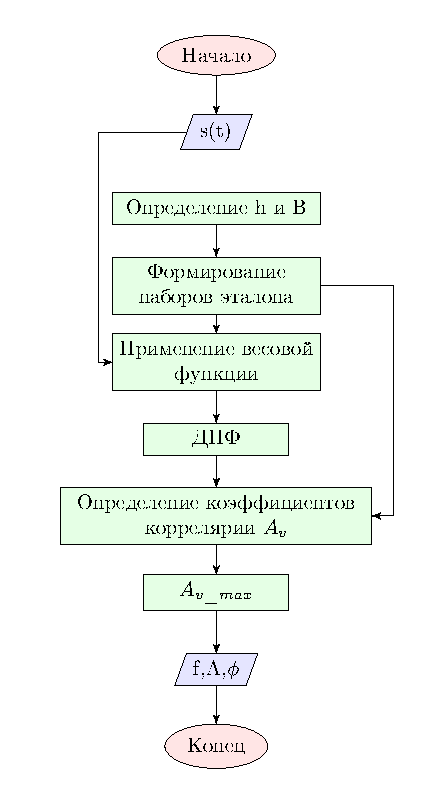
\includegraphics [scale=0.9] {GSA_Cor_fanc}
	\caption{ГСА метода корреляционных функций.}
	\label{img:picture23}
\end{figure}

Листинг программы, реализующий метод корреляционных функций, приведен в \textbf{приложении ?}. 

На \textbf{рисунке ?} представлен график смещения оценки основной частоты напряжения в зависимости от уровня шума для метода корреляционных функций.

Для метода корреляционных функций амплитуда  $\nu$-й гармоники напряжения определяется по формуле 	\ref{eq:equation3.10}. 




\section{Свертка} \label{sec:ch3/sect4}

Свертка и цифровые фильтры с конечной импульсной характеристикой (КИХ) вычисляются по формуле [1]:
% 1.	Макклеллан Дж. Х., Рейдер Ч.М. Применение теории чисел в цифровой обработке сигналов.: Радио и связь, 1983. 263 с.

\begin{equation}
	\label{eq:y(n)}
	y(n) = \sum_{k=0}^{L-1}x(n-k)h(k)
\end{equation}

где $x(n)$ -- входной сигнал;

$y(n)$ -- выходной сигнал; 

$N$ -- длина сигнала x;

$h(n)$ -- импульсный отклик системы, длиной $L$. 

В случае, если длина выходного сигнала $y(n)$,  рассчитанная по формуле (1), равна $(N+L-1)$ и для его вычисления по формуле (1) требует $N*L$ умножений и $(N-1)(L-1)$ сложений. 
Недостаток вычисления операции дискретной свертки по формуле (1), заключается в том, что требуется много вычислительных операций. Другой недостаток, что происходят временные задержки при обработке последовательности, поэтому используют секционирование сигнала и вычисление свертки для его блоков.
Для решения поставленной задачи рассмотрим быстрые алгоритмы. Любой алгоритм можно описывать через соотношение между входом и выходом, либо детально предоставить информацию, объясняя его внутреннюю структуру. Если считать, что заданный алгоритм вход-выход  имеет возможность  быть описанным математической формулой, то такая реализация будет называться прямой. К быстрым алгоритмам относятся вычислительные процедуры, которые не являются очевидным способом вычисления к данному входу, основное их преимущество – сокращение количества операций.  Для оценки сложности алгоритма используют количество арифметических операций (сложения, вычитания, умножение, деление). Важно различать быстрый алгоритм, функцию, которую он вычисляет, и приложение в котором используется. Например, необходимо различать дискретное преобразование Фурье (ДПФ) от быстрого преобразования Фурье (БПФ), т.~к.  второе преобразование является  алгоритмом для первого [2]. 
% 2. Блейхут Р. Быстрые алгоритмы цифровой обработки сигналов: Пер. с англ.–М.: Мир, 1989.–448 с.

Существует два подхода для вычисления свертки. Первый подход заключается в том, что входные последовательности x и y разбиваются на короткие секции(блоки) из несколько сотен отчетов. На выходе секции(блоки) обрабатываются поочередно методом циклической свертки. Следующий вид первого подхода заключается в вычислении циклической свертки алгоритмом Быстрого Преобразования Фурье или другими преобразованиями [2,4,5,6].

%2.	Блейхут Р. Быстрые алгоритмы цифровой обработки сигналов: Пер. с англ.–М.: Мир, 1989.–448 с.
%3.	Mou Z.J. Fast FIR filtering: algorithms and implementations / Z.J. Mou, P. Duhame // Signal Processing. – 1987. – Vo1. 13, № 4. – P. 377–384 с.
%4.	Рабинер Л. Теория и применение цифровой обработки сигналов / Л. Рабинер, Б. Гоулд. – М.: Мир, 1978. –848 с.
%5.	Нуссбаумер Г. Быстрое преобразование Фурье и алгоритмы вычисления сверток. – М.: Радио и связь, 1985.–248 с.
%6.	Оппенгейм А., Шафер М. Цифровая обработка сигналов. –М.: Техносфера, 2012 1048 с.

Второй подход, когда входные последовательности x и y  разбиваются на последовательности из четных и нечетных отчетов. Вычисление коротких последовательностей происходит быстрее. [3].
%3.	Mou Z.J. Fast FIR filtering: algorithms and implementations / Z.J. Mou, P. Duhame // Signal Processing. – 1987. – Vo1. 13, № 4. – P. 377–384 с.
Исследования для алгоритмов одномерной свертки производились в  среде разработке JetBrains CLion 2018.1 для языка программирования С. CLion – это интегрированная среда разработки (IDE), которая использует набор инструментов Cygwin (Unix-подобная среда и интерфейс командной строки для Microsoft Windows). 
В результате исследования быстродействия алгоритмов одномерной свертки на языке программирования С был получен график временных затрат с зависимостью длины фильтра от времени. Исходные данные: количество отчетов при изменении длины фильтра $100-900$ и длины сигнала $10000-40000$, количество опытов $10000$ раз. Быстродействие алгоритмов свертки на языке программирования С приведено на 
рисунке 1. 
Полученные графики построены с помощью библиотеки Matplotlib, которая строит высококачественные графики в Python. Данные графики были построены из табличных значений, формат файлов CSV (Comma-Separated Values). Режим Full возвращает свертку с выходной формой $N+L-1$.  $N$ и $L$ – размер одномерных входных массивов.

\begin{figure}[ht]
	\centering
	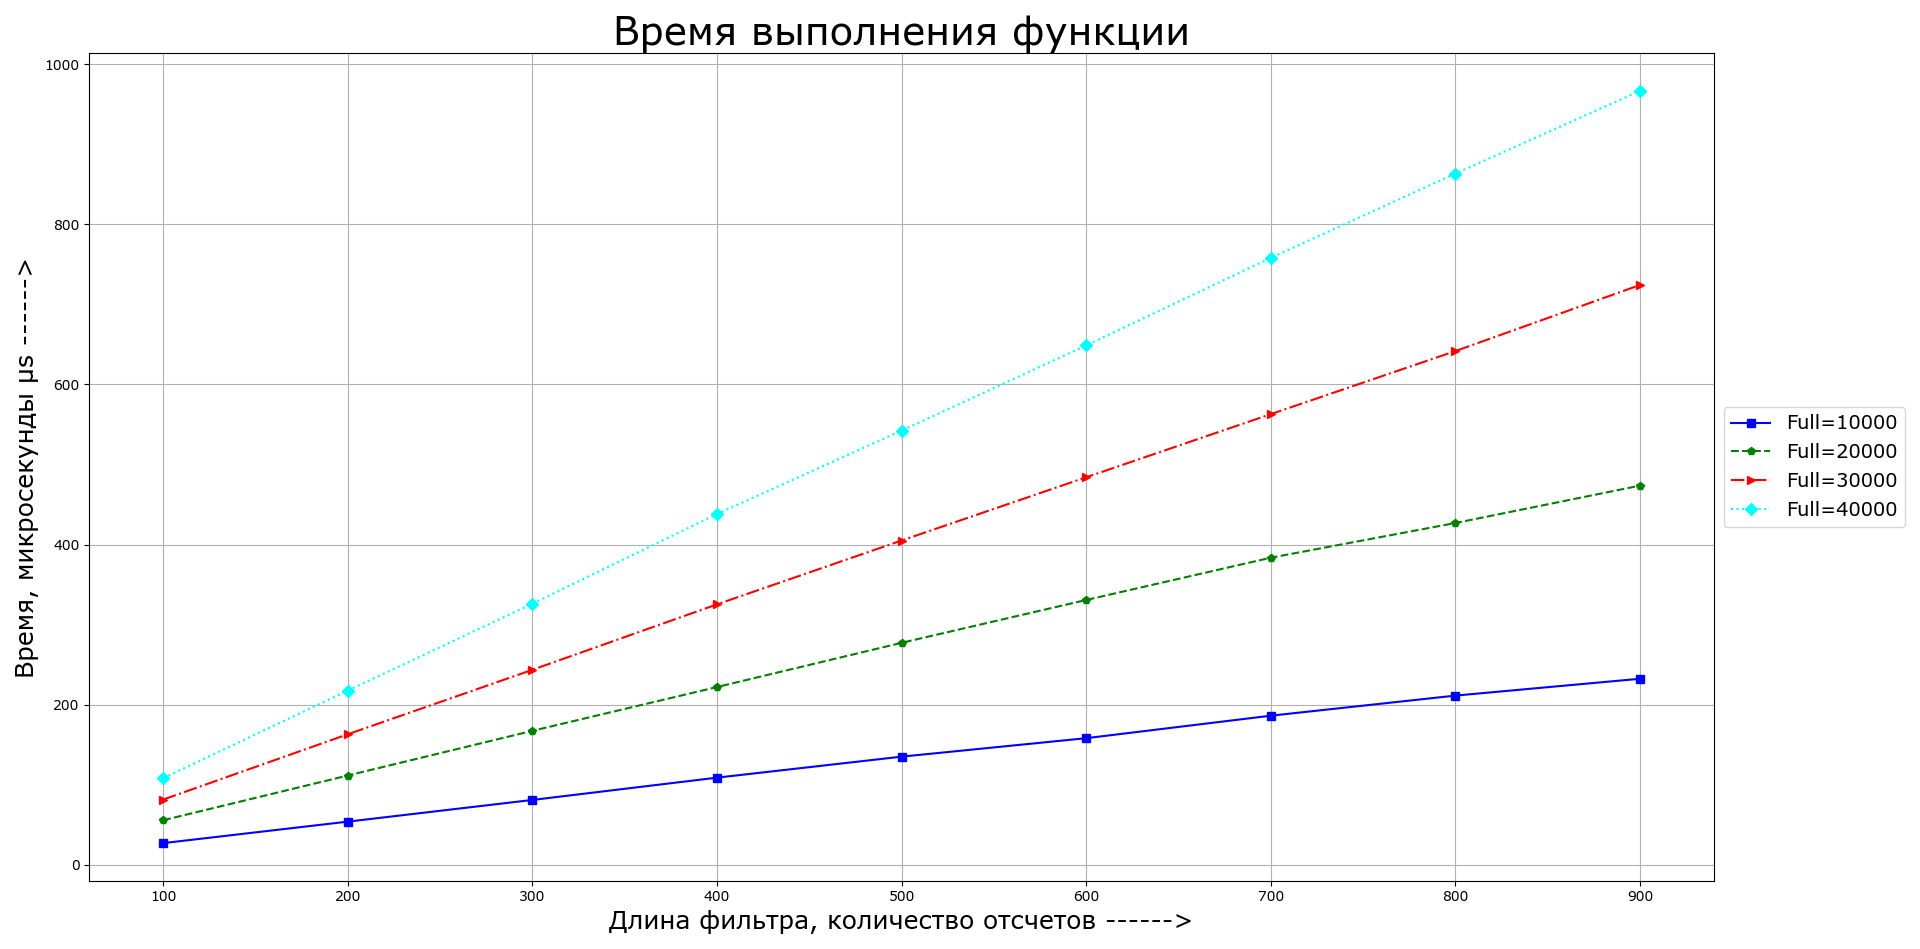
\includegraphics [scale=0.3] {convolution}
	\caption{Временные затраты на вычисление по алгоритму одномерной свертки на языке С (процессор Intel® Core™ $i5-3550$).}
	\label{img:convolution}
\end{figure}



В исследовании произведен анализ быстродействия реализаций алгоритмов одномерной свертки и цифровых фильтров. Для фильтрации  узкополосных сигналов требуются фильтры с импульсной характеристикой, содержащих большое число отчетов. 
В результате исследования была установлена необходимость минимизировать вычислительные затраты для цифровых фильтров с конечной импульсной характеристикой (рисунок 1).
Для фильтрации  узкополосных сигналов, необходимо использовать быстрые алгоритмы, т.~к. они позволяют сократить количество операций. 


\section{Интерполированный алгоритм ДПФ} \label{sec:ch3/sect5}
Интерполированный алгоритм ДПФ (IpDFT -- Interpolated Discrete Fourier Transform) является одним из наиболее широко изученных методов оценки \cite{santamaria2000comparative, zhang2001algorithm, qian2007interharmonics, ferreira2005accurate, xie1996nonlinear, luo2015phase, jain1979high, grandke1983interpolation, andria1989windows, offelli1989interpolation, agrez2002weighted, jacobsen2007fast, belega2009multifrequency, belega2010accuracy, duda2011dft, schoukens1992interpolated}. 
% [156.-Santamaria I., Pantaleon C., Ibanez J. A comparative study of high-accuracy frequency estimation methods //Mechanical Systems and Signal Processing. – 2000. – Т. 14. – №. 5. – С. 819-834.]

% [157.-Zhang F., Geng Z., Yuan W. The algorithm of interpolating windowed FFT for harmonic analysis of electric power system //IEEE transactions on power delivery. – 2001. – Т. 16. – №. 2. – С. 160-164.]

%[158.-Qian H., Zhao R., Chen T. Interharmonics analysis based on interpolating windowed FFT algorithm //IEEE Transactions on Power Delivery. – 2007. – Т. 22. – №. 2. – С. 1064-1069.]

%[159.	Ferreira A., Sinha D. Accurate and robust frequency estimation in the ODFT domain //IEEE Workshop on Applications of Signal Processing to Audio and Acoustics, 2005. – IEEE, 2005. – С. 203-206.]

%[160.-Xie M., Adams D. F. A nonlinear finite element analysis for composite materials //Finite elements in analysis and design. – 1996. – Т. 22. – №. 3. – С. 211-223.]

%[161.-Luo J., Xie M. Phase difference methods based on asymmetric windows //Mechanical Systems and Signal Processing. – 2015. – Т. 54. – С. 52-67.]

%[162.-Jain V. K., Collins W. L., Davis D. C. High-accuracy analog measurements via interpolated FFT //IEEE Transactions on Instrumentation and Measurement. – 1979. – Т. 28. – №. 2. – С. 113-122.]

% [163.-Grandke T. Interpolation algorithms for discrete Fourier transforms of weighted signals //IEEE transactions on instrumentation and measurement. – 1983. – Т. 32. – №. 2. – С. 350-355.]

%[164.-Andria G., Savino M., Trotta A. Windows and interpolation algorithms to improve electrical measurement accuracy //IEEE Transactions on Instrumentation and Measurement. – 1989. – Т. 38. – №. 4. – С. 856-863.]

%[165.-Offelli C., Petri D. Interpolation techniques for real-time multifrequency waveform analysis //6th IEEE Conference Record., Instrumentation and Measurement Technology Conference. – IEEE, 1989. – С. 325-331.]

%[166.-Agrez D. Weighted multipoint interpolated DFT to improve amplitude estimation of multifrequency signal //IEEE Transactions on Instrumentation and Measurement. – 2002. – Т. 51. – №. 2. – С. 287-292.]

%[167.-Jacobsen E., Kootsookos P. Fast, accurate frequency estimators [DSP Tips & Tricks] //IEEE Signal Processing Magazine. – 2007. – Т. 24. – №. 3. – С. 123-125.]

%[168.	Belega D., Dallet D. Multifrequency signal analysis by interpolated DFT method with maximum sidelobe decay windows //Measurement. – 2009. – Т. 42. – №. 3. – С. 420-426.]

%[169.-Belega D., Dallet D., Petri D. Accuracy of sine wave frequency estimation by multipoint interpolated DFT approach //IEEE Transactions on Instrumentation and Measurement. – 2010. – Т. 59. – №. 11. – С. 2808-2815.]

%[170.-Duda K. DFT interpolation algorithm for Kaiser–Bessel and Dolph–Chebyshev windows //IEEE Transactions on Instrumentation and Measurement. – 2011. – Т. 60. – №. 3. – С. 784-790.]

%[171.-Schoukens J., Pintelon R., Van Kamme H. The interpolated fast Fourier transform: A comparative study //[1991] Conference Record. IEEE Instrumentation and Measurement Technology Conference. – IEEE, 1991. – С. 358-364.]


Рассмотрим непрерывный сигнал с аддитивным белым шумом:
\begin{equation}
	\label{eq:$x(t)$}
	x(t) = A_0 \cos \big( 2 \pi f_0 t + \theta_0 + e(t)\big) 
\end{equation}

где $A_0$ -- амплитуда;

$f_0$ -- частота;

$\theta_0$ -- фазовый угол;

$t$ -- время;

$e(t)$ -- белый шум. 

Частота $f_s$ с интервалом $N\bigtriangleup t$, где $\bigtriangleup t = \cfrac{1}{f_s}$, $N$ -- отчеты.

По теореме Котельникова (в зарубежной литературе теорема Найквиста -- Шеннона или теорема отчетов) непрерывные и дискретные сигналы $x(t)$ состоящих из частот ($0$ до $f_0$) можно передавать с любой точностью при помощи чисел, следующих друг за другом через $\frac{1}{2f_0}$. 

\begin{equation}
	\label{eq:$x(n)$}
	x(n) = A_0 \cos(2 \pi \frac{f_0}{f_s} n + \theta_0) + e(n), n = 0,1, \cdots , N-1
\end{equation}

По теореме Котельникова, $f_s$ больше $2f_0$. Разрешающая способность по частоте $\bigtriangleup f = \cfrac{f_s}{N}$ определяется:

\begin{equation}
	\label{eq:equation14}
	\frac{f_0}{f_s}=\frac{\lambda_0}{N}
\end{equation}

$\lambda_0$ -- количество циклов или нормированная частота.


Умножим отчеты сигнала $x(n)$ на значение окна данных $\omega(n)$.

\begin{equation}
	\label{eq:equation15}
	x_\omega(n)=A_0 \cos(\frac{2 \pi \lambda_0 n}{N}+\theta_0)\omega(n)
\end{equation}

ДПФ взвешенного сигнала может быть вычислена путем:

\begin{equation}
	\label{eq:equation16}
	X_\omega(k) = \sum_{n=0}^{N-1} x_\omega(n) e^{-j \frac{2 \pi}{N}nk}
\end{equation}

Применение \labelcref{eq:equation16} к отчетам в \labelcref{eq:equation15} дает вид:

\begin{equation}
	\label{eq:equation17}
	X_\omega(k) = \frac{A_0}{2} e^{j\phi_0}W_N(k-\lambda_0)+\frac{A_0}{2}e^{j\phi_0}W_N(k+\lambda_0)
\end{equation}

где $W_N (k)$ -- дискретное временное преобразование Фурье (DTFT-- Discrete time Fourier transform) весовой функции. 

Нормированная частота $\lambda_0$ находится между двумя самыми большими спектральными линиями. Следовательно, $\lambda_0$  может быть записано с целой частью $l_\omega$ и дробной частью $\delta_\omega$ $(-0,5<\delta_{\omega}\leq0,5)$.

\begin{equation}
	\label{eq:equation18}
	\lambda_0 = l_\omega + \delta_\omega
\end{equation}

Целая часть $l_\omega$ может быть определена с помощью отношения сигнал/шум (SNR -- signal-to-noise ratio) превышает пороговое значение (приблизительно от -$18$ до –$20$ дБ) \cite{rife1974single}. 

Подстановка формулы \labelcref{eq:equation18} в \labelcref{eq:equation17}:
\begin{equation}
	\label{eq:equation19}
	\left|{X_\omega(l_\omega)} \right| = \frac{A_0}{2} \left| e^{j\phi_0}W_N(- \delta_\omega) +e^{j\phi_0}W_N(2l_\omega+\delta_\omega) \right| 
\end{equation}

Параметр $\alpha$ зависит только от выбранного окна и отклонения частоты $\delta_{\omega}$. 

\begin{equation}
	\label{eq:equation20}
	\delta_\omega = g(\alpha)
\end{equation}

Для максимальных окон распада боковых лепестков $\delta_{\omega}$ запишем как функцию от $\alpha$ в простой форме \cite{zhang2001algorithm, qian2007interharmonics, xie1996nonlinear, luo2015phase, belega2009multifrequency, belega2010accuracy}. Для других окон предлагается решение полиномиальной аппроксимации \cite{duda2011dft}. 

Рассмотрим алгоритм техники заполнения нулями. Заполнение нулями -- это метод, определяемый как добавление нулевых значений к отчетам до вычисления ДПФ. Добавленные нулевые значения обрабатываются как дополнительные отчеты, поэтому увеличивают время измерения \labelcref{eq:equation21}:

\begin{equation}
	\label{eq:equation21}
	x_{ap}(n)=
	\begin{cases}
		x_{\omega}, \leq n < N
		\\ 0, N \leq n < MN
	\end{cases}
\end{equation}

где $(M-1) \cdot N$ -- добавление нулевых значений.

Соответственно, дискретный спектр расширяется. Эта процедура приводит к более точной выборке спектра сигнала, потому что вместо $N$ спектральных отчетов $M \cdot N$. Добавление нулевых значений и вычисление более длинного ДПФ действительно увеличивает количество точек в частотной области \cite{dorf2006circuits}.

Алгоритм техники заполнения нулями не влиет на параметры спектра (отношение сигнал/шум, спектральная утечка).  Коэффициенты ДПФ по \labelcref{eq:equation21}:

\begin{equation}
	\label{eq:equation22}
	X(N)= \sum_{n=0}^{MN-1} x_{ap}(n) e^{-j \frac{2 \pi}{N}\cdot \frac{k}{M} \cdot n}, 0\leq k \leq MK-1
\end{equation}
По сравнению с \labelcref{eq:equation16} получается:

\begin{equation}
	\label{eq:equation23}
	X(k)= X_\omega \left( {\frac{k}{M}}\right)  \end{equation}
Соответственно, \labelcref{eq:equation19} можно переформулировать как:

\begin{equation}
	\label{eq:equation24}
	\left| {X(l)} \right|   = \frac{A_0}{2}\left| {e^{j\phi_0}W_N(-\delta)+e^{-j\phi_0}W_N \left(\frac{2l}{M}+\delta \right)} \right|,
\end{equation}

где $l$ и $\hat{\delta}
\left( {\delta= \frac{\hat{\delta}}{M}}\right) $
часть для $M\lambda_0$. Точно так же $l$ возвращается максимальной процедурой поиска X(k). На этом этапе три крупнейших линии $X(k)$ даны $\left| {X(l)} \right|$,$\left| {X(l+1)} \right|$ а также $\left|{X(l-1)}\right|$.

Рассмотрим алгоритм интерполяции для окна Хеннинга с техникой заполнения нулями.
Если $\lambda_0$ удовлетворяет $5<\lambda_0$ , а также $\lambda_0 < \frac{N}{2}-5$, тогда помехи от второго слагаемого могут быть минимальными и ими можно пренебречь. Поэтому \labelcref{eq:equation24} сводится к:
\begin{equation}
	\label{eq:equation25}
	\left| {X(l)} \right| \cong \frac{A_0}{2}\left| {W_N(-\delta)} \right|,
\end{equation}

Если $\left| {X(l)} \right| \cong \frac{A_0}{2}\left| {W_N(\varepsilon -\delta)} \right|$ и $\left| {X(l-1)} \right| \cong \frac{A_0}{2} \left| {W_N(\varepsilon +\delta)} \right|$, где $\varepsilon=\frac{1}{M}$. 

Для окна Хеннинга (Hanning window), $W_N (k) \cong \frac{sin(\pi k)}{h(k)}$,
$h(k) = 2 \pi k (1-k^2)$ \cite{xie1996nonlinear}
%[160.	Xie M., Adams D. F. A nonlinear finite element analysis for composite materials //Finite elements in analysis and design. – 1996. – Т. 22. – №. 3. – С. 211-223.]

\begin{equation}
	\label{eq:equation26}
	\left| {X(l)} \right| \cong \frac{A_0}{2} \frac{\sin{(\pi \delta)} }{h(\delta)} ,
\end{equation}

\begin{equation}
	\label{eq:equation27}
	\left| {X(l+1)} \right| \cong \frac{A_0}{2} \frac{\sin{(\pi \varepsilon - \pi \delta)} }{h(\varepsilon - \delta)} ,
\end{equation}

\begin{equation}
	\label{eq:equation28}
	\left| {X(l+1)} \right| \cong \frac{A_0}{2} \frac{\sin{(\pi \varepsilon + \pi \delta)} }{h(\varepsilon + \delta)}
\end{equation}

Объединим уравнения вместе (\labelcref{eq:equation27} и \labelcref{eq:equation28}):

\begin{equation}
	\label{eq:equation29}
	h(\varepsilon+\delta)\left|{X(l-1)} \right| - h(\varepsilon-\delta) \left|{X(l+1)} \right| \cong A_0 \sin{(\pi \delta)} \cos{(\pi \varepsilon)}
\end{equation}

Дальнейшее объединение \labelcref{eq:equation26} и \labelcref{eq:equation29}

\begin{equation}
	\label{eq:equation30}
	h(\delta+\varepsilon)\left|{X(l-1)} \right| - h(\delta - \varepsilon) \left|{X(l+1)} \right| \cong 2 \left|{X(l)} \right| h(\delta) \cos{(\pi \varepsilon)}
\end{equation}

Теперь введем две переменные $\gamma_1$,$\gamma_2$ определяются как:

\begin{equation}
	\label{eq:equation31}
	\gamma_1 = \frac{\left| X(l-1)\right|}{\left| X(l)\right|}
\end{equation}

\begin{equation}
	\label{eq:equation32}
	\gamma_1 = \frac{\left| X(l+1)\right|}{\left| X(l)\right|}
\end{equation}

Для простоты и краткости будем использовать знак $«=»$ в \labelcref{eq:equation30}, вместо $\cong$. Но отношение аппроксимации остаются. 

\begin{equation}
	\label{eq:equation33}
	h(\delta +\varepsilon)\gamma_1 - h(\delta -\varepsilon)\gamma_2 = 
	2h(\delta) \cos(\pi \varepsilon) 
\end{equation}

При условии $h(\delta +\varepsilon)$,$h(\delta -\varepsilon)$ получаем:

\begin{equation}
	\label{eq:equation34}
	{a \delta}^3 + {b \delta}^2 + c \delta + d = 0, 
\end{equation}

где $a = 2 \cos(\pi \varepsilon)-(\gamma_1 + \gamma_2)$;

$b = -3(\gamma_1 - \gamma_2)\varepsilon$;

$c = \left( \gamma_1 + \gamma_2 - \frac{2 \cos(\pi \varepsilon)}{1-3\varepsilon^2}
\right) \left( {1-3\varepsilon^2} \right) $;

$d = ( \gamma_1 - \gamma_2)(\varepsilon - \varepsilon^3)$

\begin{equation}
	\label{eq:equation35}
	g(\delta) = {a \delta}^3 + {b \delta}^2 + c \delta + d
\end{equation}

Можно доказать, что $g(-1)>0$,$g(-0,5)<0$,$g(0,5)>0$,$g(1)<0$ 

\begin{equation}
	\label{eq:equation36}
	\gamma_1 = \frac{\left| X(l-1)\right|}{\left| X(l)\right|} = \frac{\sin({\pi \varepsilon + \pi \delta})}{h(\varepsilon + \delta)} \cdot \frac{h(\delta)}{\sin(\pi \delta)}
\end{equation}

\begin{equation}
	\label{eq:equation37}
	\gamma_2 = \frac{\left| X(l+1)\right|}{\left| X(l)\right|} = \frac{\sin({\pi \varepsilon - \pi \delta})}{h(\varepsilon - \delta)} \cdot \frac{h(\delta)}{\sin(\pi \delta)}
\end{equation}

где $\delta \in[-0.5,0.5]$ а также $\varepsilon\in[0,0.5]$. Согласно формуле \labelcref{eq:equation35}

\begin{equation}
	\label{eq:equation38}
	f(0,5) = -\frac{3}{4} \cos(\pi \varepsilon) + \frac{(1-4 \varepsilon^2)}{8} \left[ {\gamma_1 (3+2 \varepsilon)+\gamma_2 (3-2 \varepsilon)}\right] 
\end{equation}

\begin{equation}
	\label{eq:equation39}
	f(-0,5) = +\frac{3}{4} \cos(\pi \varepsilon) + \frac{(1-4 \varepsilon^2)}{8} \left[ {\gamma_1 (3-2 \varepsilon)+\gamma_2 (3+2 \varepsilon)}\right] 
\end{equation}

\begin{equation}
	\label{eq:equation40}
	f(1) = -\gamma_1 \varepsilon(\varepsilon+1)(\varepsilon + 2) + \gamma_2 \varepsilon(\varepsilon-1)(\varepsilon - 2)
\end{equation}

\begin{equation}
	\label{eq:equation41}
	f(-1) = -\gamma_1 \varepsilon(\varepsilon-1)(\varepsilon - 2) + \gamma_2 \varepsilon(\varepsilon+1)(\varepsilon + 2)
\end{equation}

Определяем $p(\delta)$:

\begin{equation}
	\label{eq:equation42}
	p(\delta) = \gamma_1 (3+2\varepsilon) + \gamma_2 (3-2\varepsilon)
\end{equation}

Определяем $q(\delta)$:
\begin{equation}
	\label{eq:equation43}
	q(\delta) = \gamma_1 (3-2\varepsilon) + \gamma_2 (3+2\varepsilon)
\end{equation}

$p(\delta)$ является монотонно возрастающей функцией. Поэтому:
\begin{equation}
	\label{eq:equation44}
	p_{min}(\delta) = p(\delta = 0,5) = \frac{6 \cos(\pi  \varepsilon)}{1-4\varepsilon ^2}
\end{equation}

также
\begin{equation}
	\label{eq:equation45}
	q_{min}(\delta) = q(\delta = -0,5) = \frac{6 \cos(\pi  \varepsilon)}{1-4\varepsilon ^2}
\end{equation}

Тогда
\begin{equation}
	\label{eq:equation46}
	f(0,5) > -\frac{3}{4} \cos (\pi \varepsilon) + \frac{(1-4 \varepsilon ^2)}{8} p_{min} (\delta) = - \frac{3}{4} \cos(\pi \varepsilon) + \frac{3 \ cos(\pi \varepsilon)}{4} = 0 
\end{equation}

\begin{equation}
	\label{eq:equation47}
	f(-0,5) < \frac{3}{4} \cos (\pi \varepsilon) + \frac{(1-4 \varepsilon ^2)}{8} q_{min} (\delta) = + \frac{3}{4} \cos(\pi \varepsilon) - \frac{3 \ cos(\pi \varepsilon)}{4} = 0 
\end{equation}

Определим:
\begin{equation}
	\label{eq:equation48}
	u(\varepsilon, \gamma) = \frac{f(1)}{\varepsilon \gamma_1} = (\varepsilon ^2 + 2) (\gamma - 1) - 3\varepsilon (\gamma + 1)
\end{equation}

\begin{equation}
	\label{eq:equation49}
	\nu(\varepsilon, \gamma) = \frac{f(-1)}{\varepsilon \gamma_1} = (\varepsilon ^2 + 2) (\gamma - 1) + 3\varepsilon (\gamma + 1)
\end{equation}

$\gamma = \frac{\gamma_1}{\gamma_2}$

\begin{equation}
	\label{eq:equation50}
	u'_{\gamma}(\varepsilon, \gamma) = \varepsilon^2 - 3\varepsilon + 2 = (\varepsilon - 2)(\varepsilon -1) >0
\end{equation}

\begin{equation}
	\label{eq:equation51}
	{\nu}'_\gamma
	(\varepsilon, \gamma) = \varepsilon^2 + 3\varepsilon + 2 = (\varepsilon + 2)(\varepsilon + 1) >0
\end{equation}


\begin{equation}
	\label{eq:equation52}
	u _{max}(\varepsilon, \gamma) =
	\left( {\varepsilon^2+2} \right) 
	\left( {\frac{1,5+\varepsilon}{1,5-\varepsilon}-1} \right) - 3 \varepsilon 
	\left( {\frac{1,5+\varepsilon}{1,5-\varepsilon}+1} \right) = \frac{\varepsilon}{1,5-\varepsilon}(2\varepsilon^2 - 5) < 0
\end{equation}

\begin{equation}
	\label{eq:equation53}
	\nu _{min}(\varepsilon, \gamma) =
	\left( {\varepsilon^2+2} \right) 
	\left( {\frac{1,5-\varepsilon}{1,5+\varepsilon}-1} \right) - 3 \varepsilon 
	\left( {\frac{1,5-\varepsilon}{1,5+\varepsilon}+1} \right) = \frac{\varepsilon}{1,5-\varepsilon}(5-2\varepsilon^2) > 0
\end{equation}

Соответственно:

\begin{equation}
	\label{eq:equation54}
	f(1) = u(\varepsilon, \gamma)(\varepsilon \gamma_1) <0
\end{equation}

\begin{equation}
	\label{eq:equation55}
	f(-1) = \nu(\varepsilon, \gamma)(\varepsilon \gamma_1) > 0
\end{equation}

Согласно исследованию в \cite{nickalls1993new}, корни можно выразить:

%[174.	Nickalls R. W. D. A new approach to solving the cubic: Cardan’s solution revealed //The Mathematical Gazette. – 1993. – Т. 77. – №. 480. – С. 354-359.]

\begin{equation}
	\label{eq:equation56}
	\delta_1 = 
	\delta_0 + 2 \sigma \cos \left({\frac{2 \pi}{3}} + \varphi  \right) 
\end{equation}

\begin{equation}
	\label{eq:equation57}
	\delta_2 = 
	\delta_0 + 2 \sigma \cos \left({\frac{2 \pi}{3}} - \varphi  \right) 
\end{equation}

\begin{equation}
	\label{eq:equation58}
	\delta_3 = 
	\delta_0 + 2 \sigma \cos (\varphi) 
\end{equation}

$\delta_0 = \frac{-a}{3b};$

$\sigma = \sqrt{\frac{b^2 - 3ac}{9a^2}}$

$\cos(3 \varphi) = - g \left( {\frac{\delta_0}{p}}
\right) $

$p = -a \delta_0 ^3$

$\delta_1$ и $\delta_3$ выходят за пределы определенного диапазона $(-0,5;0,5]$. Таким образом, единственным решением является $\delta_2 $. Получаем:

\begin{equation}
	\label{eq:equation59}
	\hat{\delta} = \delta_2 + \delta_0 + 2 \sigma \cos \left({\frac{2 \pi}{3} - \varphi} \right) 
\end{equation}

Рассмотрим расширение на другие классические окна .

Расширим интерполяцию для других классических окон, используя метод подгонки основного лепестка. 

\begin{equation}
	\label{eq:equation60}
	S(k) = [W_C (k)]^q - W_H (k)
\end{equation}

где $W_C (k)$ -- обозначает нормализованный спектр любого классического окна;

$W_H (k)$ -- обозначает нормализованный спектр окна Хеннинга;

$q = \frac{S L_{Han}}{S L_\omega(n)}$

$S L_{Han}$ и $S L_\omega(n)$ -- представляют собой убывающие потери $SL$ окна Хеннинга.

Можно определить, что $|S(k)|$ очень мало 
для большинства классических окон, если $k$ находится в диапазоне  $(-0,5;0,5]$. 
Например, максимальное значение $|S(k)|$ равняется $10-5$ для окна Хемминга(Hamming window) и $10^-4$ для окна Блэкмена (Blackman window).
Означает, что $[W_C (k)]^q$, а также $W_H (k)$ хорошо сочетаются друг с другом в середине их основных лепестков. 
Подразумевается, что вышеуказанный алгоритм интерполяции может быть расширен для классических окон, пока $[W_C (k)]^q$ используется $k$ и ограничен в диапазоне $[-0,5;0,5]$. 
С техникой заполнения нулями $(M\geq3)$, три самые большие спектральные линии, которые используются в алгоритме интерполяции, легко удовлетворяют требованию. Для большого $M$, погрешность оценки будет уменьшаться как в шуме, так и в ситуации без шума. Однако улучшение не ясно, когда $(M>5)$. С другой стороны, объем расчета увеличится из-за добавленного нуля. Следовательно, учитывая объем вычислений и алгоритм БПФ для radix-2, часто выбираем $(M=4)$ для практических измерений.

Согласно определению в уравнениях \labelcref{eq:equation31} и \labelcref{eq:equation32}, имеем

\begin{equation}
	\label{eq:equation62}
	\gamma_1 = \frac{\left| X(l-1)\right|}{\left| X(l)\right|} = \frac{\sin \pi({\delta + \varepsilon})}{\sin \pi \delta} \cdot \frac{h(\delta)}{h(\delta + \varepsilon)}
\end{equation}

\begin{equation}
	\label{eq:equation63}
	\gamma_2 = \frac{\left| X(l+1)\right|}{\left| X(l)\right|} = \frac{\sin \pi({\delta - \varepsilon})}{\sin \pi \delta} \cdot \frac{h(\delta)}{h(\delta - \varepsilon)}
\end{equation}

\begin{equation}
	\label{eq:equation64}
	\gamma = \frac{\left| X(l+1)\right|}{\left| X(l-1)\right|} = \frac{\sin \pi({\delta - \varepsilon})}{\sin \pi ({\delta + \varepsilon})} \cdot \frac{h({\delta + \varepsilon})}{h(\delta - \varepsilon)}
\end{equation}

Знаем $\gamma_1$, является монотонно убывающей функцией и $\gamma_2$, $\gamma$ является монотонно возрастающей функцией в зависимости от $\delta$ в диапазоне $[-0.5;0.5]$. Итак, можем получить

\begin{equation}
	\label{eq:equation65}
	\gamma_{1 max} = \gamma_1 (\delta = - 0,5) = \frac{3 \cos \pi \varepsilon}{(1 + 2 \varepsilon)(1 - 2 \varepsilon)(3 - 2 \varepsilon)}
\end{equation}

\begin{equation}
	\label{eq:equation66}
	\gamma_{1 min} = \gamma_1 (\delta = 0,5) = \frac{3 \cos \pi \varepsilon}{(1 + 2 \varepsilon)(1 - 2 \varepsilon)(3 + 2 \varepsilon)}
\end{equation}

\begin{equation}
	\label{eq:equation67}
	\gamma_{2 max} = \gamma_2 (\delta = 0,5) = \frac{3 \cos \pi \varepsilon}{(1 + 2 \varepsilon)(1 - 2 \varepsilon)(3 - 2 \varepsilon)}
\end{equation}

\begin{equation}
	\label{eq:equation68}
	\gamma_{2 min} = \gamma_2 (\delta = -0,5) = \frac{3 \cos \pi \varepsilon}{(1 + 2 \varepsilon)(1 - 2 \varepsilon)(3 + 2 \varepsilon)}
\end{equation}

\begin{equation}
	\label{eq:equation69}
	\gamma_{max} = \gamma(\delta = 0,5) = \frac{1,5+ \varepsilon}{1,5 - \varepsilon}
\end{equation}

\begin{equation}
	\label{eq:equation70}
	\gamma_{min} = \gamma(\delta = -0,5) = \frac{1,5 - \varepsilon}{1,5 + \varepsilon}
\end{equation}

Согласно бесконечному представлению Эйлера функции синуса:

\begin{equation}
	\label{eq:equation71}
	\sin \pi \delta = \pi \delta \prod\limits_{n = 1}^\infty \left( 1- \frac{\delta^2}{n^2} \right) 
\end{equation}

\begin{equation}
	\label{eq:equation72}
	E(\delta) = \frac{\sin(\pi \delta) }{h(\delta)} = \frac{\pi \delta \prod\limits_{n = 1}^\infty \left( 1- \frac{\delta^2}{n^2}\right)}{\pi \delta (1 - \delta^2)} = \prod\limits_{n = 2}^\infty \left( 1 - \frac{\delta^2}{n^2}\right) \geq 0 
\end{equation}

Находим производную $E(\delta)$:     

\begin{equation}
	\label{eq:equation73}
	E'(\delta) = E(\delta)L(\delta)
\end{equation}

\begin{equation}
	\label{eq:equation74}
	L(\delta) = \sum_{n=2}^{\infty} \frac{-2 \delta}{n^2 - \delta^2} = \sum_{n=2}^{\infty} \left(  \frac{1}{n + \delta} -  \frac{1}{n - \delta} \right) 
\end{equation}

\begin{equation}
	\label{eq:equation75}
	D(\delta) = \frac{E(\delta)}{E(\delta + \epsilon)} = \frac{\prod\limits_{n = 2}^\infty \left( 1 - \frac{\delta^2}{n^2} \right) }{\prod\limits_{n = 2}^\infty \left( \frac{1 - (\delta + \epsilon)^2}{n^2}\right)} = \prod\limits_{n = 2}^\infty \frac{n^2 - \delta^2}{n^2 - (\delta + \epsilon)^2}
\end{equation}

\begin{equation}
	\label{eq:equation76}
	D'(\delta) = \frac{E(\delta)L(\delta)E(\delta + \epsilon) - E(\delta)E(\delta + \epsilon)L(\delta + \epsilon)}{E^2 (\delta + \epsilon)} = \frac{E(\delta) [L(\delta) - L(\delta + \epsilon)])}{E(\delta + \epsilon)}
\end{equation}

\begin{equation}
	\label{eq:equation77}
	L(\delta) - L(\delta + \epsilon) = \sum_{n=2}^{\infty} \left(  \frac{\epsilon}{(n + \delta)(n + \delta + \epsilon)} + \frac{\epsilon}{(n - \delta)(n - \delta - \epsilon)} \right) > 0
\end{equation}

\begin{equation}
	\label{eq:equation78}
	D'(\delta) > 0 
\end{equation}

$D(\delta)$ -- монотонно возрастающая функция в зависимости от $\delta$, $\frac{1}{D(\delta)}$ -- монотонно убывающая функция. 

На основании уравнения \labelcref{eq:equation72} $\gamma_1, \gamma_2$ могут быть представлены:

\begin{equation}
	\label{eq:equation79}
	\gamma_1 = \frac{E(\delta + \epsilon)}{E(\delta)} 
\end{equation}

\begin{equation}
	\label{eq:equation80}
	\gamma_2 = \frac{E(\delta - \epsilon)}{E(\delta)} 
\end{equation}

\begin{equation}
	\label{eq:equation81}
	p(\delta) = \frac{[E(\delta + \epsilon)(3 + 2 \epsilon) + E(\delta - \epsilon)(3 - 2 \epsilon)]}{E(\delta)}
\end{equation}

\begin{equation}
	\label{eq:equation82}
	q(\delta) = \frac{[E(\delta + \epsilon)(3 - 2 \epsilon) + E(\delta - \epsilon)(3 + 2 \epsilon)]}{E(\delta)}
\end{equation}

\begin{equation}
	\label{eq:equation83}
	p'(\delta) = \frac{H_{p}(\delta, \epsilon)}{E(\delta)}
\end{equation}

\begin{equation}
	\label{eq:equation84}
	q'(\delta) = \frac{H_{q}(\delta, \epsilon)}{E(\delta)}
\end{equation}

Где $H_{p}(\delta, \epsilon)$ и $H_{q}(\delta, \epsilon)$ соответственно:

\begin{equation}
	\label{eq:equation85}
	H_{p}(\delta, \epsilon) = E(\delta + \epsilon)(3 + 2 \epsilon) [L (\delta + \epsilon) - L(\delta)] + E(\delta - \epsilon)(3 - 2\epsilon) [L(\delta - \epsilon) - L(\delta)]
\end{equation}

\begin{equation}
	\label{eq:equation86}
	H_{q}(\delta, \epsilon) = E(\delta + \epsilon)(3 - 2 \epsilon) [L (\delta + \epsilon) - L(\delta)] + E(\delta - \epsilon)(3 + 2\epsilon)[L(\delta - \epsilon) - L(\delta)]
\end{equation}

\begin{equation}
	\label{eq:equation87}
	H_{p}(\delta, \epsilon) + H_{p}(- \delta, \epsilon) = 4 \epsilon E (\delta + \epsilon) [L(\delta + \epsilon) - L(\delta)] + 4 \epsilon E (\delta - \epsilon)[L(\delta) - L (\delta - \epsilon)] 
\end{equation}

\begin{equation}
	\label{eq:equation88}
	H_{q}(\delta, \epsilon) + H_{q}(- \delta, \epsilon) = - 4 \epsilon E (\delta + \epsilon) [L(\delta + \epsilon) - L(\delta)] - 4 \epsilon E (\delta - \epsilon)[L(\delta) - L (\delta - \epsilon)]  
\end{equation}

Если $L (\delta - \epsilon) - L(\delta) < 0$ и $L(\delta) - L(\delta - \epsilon) < 0$, то:

\begin{equation}
	\label{eq:equation89}
	H_{p}(\delta, \epsilon) + H_{p}(- \delta, \epsilon) < 0  
\end{equation}

\begin{equation}
	\label{eq:equation90}
	H_{q}(\delta, \epsilon) + H_{q}(- \delta, \epsilon) > 0  
\end{equation}

\begin{equation}
	\label{eq:equation91}
	H_{p}(\delta, \epsilon) < 0
\end{equation}

\begin{equation}
	\label{eq:equation92}
	H_{q}(\delta, \epsilon) > 0
\end{equation}

\begin{equation}
	\label{eq:equation93}
	p'(\delta) = \frac{H_{p}(\delta, \epsilon)}{E(\delta)} < 0
\end{equation}

\begin{equation}
	\label{eq:equation94}
	q'(\delta) = \frac{H_{q}(\delta, \epsilon)}{E(\delta)} > 0
\end{equation}

где $p(\delta)$ -- убывающая функция;

$\delta$ -- убывающая функция;

$q(\delta)$ -- возрастающая функция.

\begin{equation}
	\label{eq:equation95}
	I(\delta, \epsilon) = \frac{E(\delta - \epsilon)}{E(\delta + \epsilon)} \cdot \frac{L(\delta - \epsilon) - L(\delta)}{L(\delta) - L(\delta + \epsilon)}
\end{equation}

\begin{equation}
	\label{eq:equation96}
	K(\epsilon) = \frac{3 + 2\epsilon}{3 - 2\epsilon}
\end{equation}

Если $I(\delta, \epsilon) > 0$, $0 < K(\epsilon) < 1 < K (\epsilon)$, а также $K(- \epsilon)K(\epsilon) = 1$.

\begin{equation}
	\label{eq:equation97}
	\frac{H_{p}(\delta, \epsilon)}{H_{p}(- \delta, \epsilon)} = \frac{I(\delta, \epsilon) - K(\epsilon)}{K(- \epsilon) - I(\delta, \epsilon)}
\end{equation}

\begin{equation}
	\label{eq:equation98}
	\frac{H_{q}(\delta, \epsilon)}{H_{q}(- \delta, \epsilon)} = \frac{K(- \epsilon) -  I(\delta, \epsilon)}{I(\delta, \epsilon) - K(\epsilon)}
\end{equation}

Если $\delta > 0$, то:
\begin{equation}
	\label{eq:equation99}
	K(- \epsilon) < \frac{E(\delta + \epsilon)}{E(\delta - \epsilon)}
\end{equation}

\begin{equation}
	\label{eq:equation100}
	1 < \frac{L(\delta) - L(\delta + \epsilon)}{L(\delta - \epsilon) - L(\delta)} < K(\epsilon)
\end{equation}

\begin{equation}
	\label{eq:equation101}
	K(- \epsilon) < I(\delta, \epsilon) < K(\epsilon)
\end{equation}

Подставив уравнение \labelcref{eq:equation101} в  \labelcref{eq:equation97} и  \labelcref{eq:equation98}, то $\frac{H_{p}(\delta, \epsilon)}{H_{p}(- \delta, \epsilon)} > 0$, а также $\frac{H_{q}(\delta, \epsilon)}{H_{q}(- \delta, \epsilon)} > 0$

\begin{equation}
	\label{eq:equation102}
	T(\delta,  \epsilon) = \frac{L(\delta) - L(\delta + \epsilon)}{L(\delta - \epsilon) - L(\delta)} \cdot \frac{ \sum_{n = 2}^{\infty} a_{n}}{\sum_{n = 2}^{\infty} b_{n}}
\end{equation}

\begin{equation}
	\label{eq:equation103}
	a_{n} = \frac{1}{(n + \delta)(n + \delta - \epsilon)} + \frac{1}{(n - \delta)(n - \delta - \epsilon)} 
\end{equation}

\begin{equation}
	\label{eq:equation104}
	b_{n} = \frac{1}{(n + \delta)(n + \delta - \epsilon)} + \frac{1}{(n - \delta)(n - \delta + \epsilon)} 
\end{equation}

\begin{equation}
	\label{eq:equation105}
	C_{n} = \frac{a_{n}}{b_{n}} = \frac{n^2 -\delta^2 - \epsilon^2 + 2\delta \epsilon}{n^2 -\delta^2 - \epsilon^2 - 2\delta \epsilon} \cdot \frac{n^2 + \delta^2 + \delta \epsilon}{n^2 + \delta^2 - \delta \epsilon}
\end{equation}

Если $\delta > 0$, $\frac{n^2 - \delta^2 - \epsilon^2 +2\delta \epsilon}{n^2 - \delta^2 - \epsilon^2 - 2\delta \epsilon} > 1$ также $\frac{n^2 + \delta^2 + \delta \epsilon}{n^2 + \delta^2 - \delta \epsilon} > 1$, то:

\begin{equation}
	\label{eq:equation106}
	C_{n} > C_{n + 1} > 1 
\end{equation}

\begin{equation}
	\label{eq:equation107}
	1 < T(\delta, \epsilon) < C_{2}
\end{equation} 

$C_{n}$ может быть записана:
\begin{equation}
	\label{eq:equation108}
	C = \frac{1 + \frac{2 \delta \epsilon}{(n^2 - \delta^2 - \epsilon^2)}}{1 - \frac{2 \delta \epsilon}{(n^2 - \delta^2 - \epsilon^2)}} \cdot \frac{1 + \frac{\delta \epsilon}{(n^2 + \delta^2)}}{1 - \frac{\delta \epsilon}{(n^2 + \delta^2)}}
\end{equation} 

Вводя параметр $D_{1} =  \frac{2 \delta \epsilon}{(n^2 - \delta^2 - \epsilon^2)}$ и $D_{1} =  \frac{\delta \epsilon}{n^2 + \delta^2}$

\begin{equation}
	\label{eq:equation109}
	C_{n} = \frac{1 + D_{1}}{1 - D_{1}} \cdot  \frac{1 + D_{2}}{1 - D_{2}} = \frac{1 + D_{1}D_{2} + D_{1} + D_{2}}{1 + D_{1}D_{2} - D_{1} - D_{2}} = \frac{1 + \frac{(D_{1} + D_{1})}{(1 + D_{1}D_{2})}}{1 - \frac{(D_{1} + D_{1})}{(1 + D_{1}D_{2})}}
\end{equation} 

\begin{equation}
	\label{eq:equation110}
	D = \delta \epsilon \frac{3n^2 - \epsilon^2 + \delta^2}{(n^2 - \delta^2 - \epsilon ^2)(n^2 + \delta ^2) + 2 \delta ^2 \epsilon^2} < \delta \epsilon \frac{3 n^2 + \frac{1}{4}}{(n^2 - \frac{1}{2})n^2}
\end{equation} 

Если $n = 2$, то
\begin{equation}
	\label{eq:equation111}
	D < \epsilon \ frac{6 + \frac{1}{8}}{14} < \frac{2}{3} \epsilon
\end{equation} 

Соответственно:
\begin{equation}
	\label{eq:equation112}
	1 < T(\delta, \epsilon) < C_{2} < \frac{1 + \frac{2 \epsilon}{3}}{1 - \frac{2 \epsilon}{3}} = K(\epsilon)
\end{equation} 

При $\delta <0$ получаем $K(\epsilon) < T(\delta, \epsilon) < 1$ 

\section{Разряженное Быстрое Преобразование Фурье} \label{sec:ch3/sect6}
% ПЕРЕПИСАТЬ СВОИМИ СЛОВАМИ

Spare FFT (SFFT, разряженное БПФ) -- алгоритм оценки спектра сигнала, содержащего малое число гармоник. В отличие от усеченного БПФ, которое находит небольшое число гармоник с заранее известным номером, SFFT находит гармоники, которые имеют более высокую амплитуду по сравнению с другими гармониками. Еще более существенное отличие SFFT от остальных БПФ заключается в том, что этот алгоритм является вероятностным и работает только для сигналов, для которых выполняются определенные условия (отсутствие в спектре большое числа гармоник с большой амплитудой, низкий уровень шума и другие).

SFFT является относительно новым подходом к вычислению спектра.
Первые публикации с идеями, лежащими в основе этого подхода, появились в
середине 90-х годов XX века \cite{kushilevitz1993learning}, после чего начали интенсивно появляться
новые алгоритмы для реализации этих идей \cite{hassanieh2012faster, hassanieh2012nearly, pawar2013computing, schumacher2014high, hassanieh2012simple}.
% Kushilevitz E., Mansour Y. Learning decision trees using the Fourier spectrum //SIAM Journal on Computing. – 1993. – Т. 22. – №. 6. – С. 1331-1348.
% Hassanieh H. et al. Faster GPS via the sparse Fourier transform //Proceedings of the 18th annual international conference on Mobile computing and networking. – 2012. – С. 353-364.
% Hassanieh H. et al. Nearly optimal sparse Fourier transform //Proceedings of the forty-fourth annual ACM symposium on Theory of computing. – 2012. – С. 563-578.
% Pawar S., Ramchandran K. Computing a k-sparse n-length discrete fourier transform using at most 4k samples and o (k log k) complexity //2013 IEEE International Symposium on Information Theory. – IEEE, 2013. – С. 464-468.
% Schumacher J., Püschel M. High-performance sparse fast Fourier transforms //2014 IEEE Workshop on Signal Processing Systems (SiPS). – IEEE, 2014. – С. 1-6.
% Hassanieh H. et al. Simple and practical algorithm for sparse Fourier transform //Proceedings of the twenty-third annual ACM-SIAM symposium on Discrete Algorithms. – Society for Industrial and Applied Mathematics, 2012. – С. 1183-1194.

Основное достоинство SFFT заключается в скорости его работы при большом числе входных данных. Он может успешно применяться для анализа сигналов в таких областях, как машинное обучение, GPS трекинг, компьютерная томография и другие.


Несмотря на обилие алгоритмов SFFT, общие принципы их работы похожи. Все алгоритмы выполняют оценку гармоник в два этапа:

\begin{itemize}
\item выполняется процедура, традиционно называемая HashToBins, которая хэширует сигнал в несколько корзин (bin) (подробнее поясним ниже);
\item выполняется процедура оценки частот.
\end{itemize}

При хэшировании сигналов в несколько корзин выполняются следующие действия:
% Что такое хэширование?
\begin{itemize}
\item отчеты входного сигнала случайным образом распределяются между $B$ корзинами;
\item отчеты, относящиеся к одной корзине, умножаются на некоторую
оконную функцию (фильтр);
\item внутри каждой корзины отчеты объединяются в группы, внутри группы отчеты суммируются;
\item выполняется B БПФ над полученными в каждой корзине суммами.

Количество корзин, оконная функция и размеры групп внутри корзин определяются в разных алгоритмах по-разному. Функция HashToBins может выполняться повторно с уточненными параметрами после второго этапа работы SFFT.
\end{itemize}

Процедура оценки частот сильно отличается от алгоритма к алгоритму, но обычно в ней присутствуют два этапа: оценка возможных позиций расположения гармоник и расчет значений этих гармоник.

Наибольших успехов в получение алгоритмов с низкой оценкой сложности достигла исследовательская группа из Массачусетского технологического института \cite{bottazzi2018new}. 
% Bottazzi G., Italiano G. F., Rutigliano G. G. A New Scalable Botnet Detection Method in the Frequency Domain //Cyber Criminology. – Springer, Cham, 2018. – С. 141-166.
Сложность предложенных ими алгоритмов составляет $O(K \log_{2} N)$ для расчета K гармоник сигнала по N входным отсчетами (если входной сигнал содержит не более K гармоник) и $O(K log_{2} N log_{2} \frac{N}{K})$ в общем случае \cite{indyk2014sparse, indyk2014nearly}.
% Indyk P., Kapralov M. Sparse Fourier Transform in Any Constant Dimension with Nearly-Optimal Sample Complexity in Sublinear Time. – 2014.
% Indyk P., Kapralov M., Price E. (Nearly) sample-optimal sparse Fourier transform //Proceedings of the Twenty-Fifth Annual ACM-SIAM Symposium on Discrete Algorithms. – Society for Industrial and Applied Mathematics, 2014. – С. 480-499.

Быстрые реализации SFFT для современных процессоров с набором SIMD инструкций были получены с помощью автоматического генератора кода проекта SPIRAL \cite{schumacher2014high, spiral}.
% Schumacher J., Püschel M. High-performance sparse fast Fourier transforms //2014 IEEE Workshop on Signal Processing Systems (SiPS). – IEEE, 2014. – С. 1-6.


На рис. 4.17 (взят с сайта http://www.spiral.net/software/sfft.html) приведены
экспериментальные результаты оценки производительности SFFT по сравнению с классическим БПФ.
На нем по вертикальной оси отложено время выполнения FFT - $N^{22}$,
по горизонтальной — количество ненулевых частот K. Вертикальные линии
показывают время выполнения БПФ с помощью одной из наиболее оптимизированных
библиотек для классического БПФ. Верхняя линия — время работы алгоритма SFFT для случая, когда в сигнале заведомо присутствует не более $K$ гармоник, нижняя линия — в общем случае.

%Рис. 4.17. Производительность разреженного преобразования Фурье

Как видно из графика, выигрыш в производительности РБПФ при большом числе точек во входном сигнале и
малом числе гармоник может быть в несколько тысяч раз.
 
%%%%%%%%%%%%%%%%
Разряженное быстрое преобразование Фурье (SFFT, Sparse Fast Fourier Transform) -- алгоритм разработанный Хайтамом Хассани (Haitham Hassanieh) и другими \cite{hassanieh2012simple} для вычисления сигналов с разреженной частотной областью. Алгоритм улучшает асимптотическое время по сравнению с другими алгоритмами \cite{hassanieh2012nearly}.

Реализация SFFT на сайте http://groups.csail.mit.edu/netmit/sFFT/
доказывает, что алгоритм быстрее, чем FFT. Однако реализация SFFT не оптимизирована для современных аппаратных функций(иерархия кэша, многопоточность, наборы векторных инструкций).

На графике показано сравнение эталонной реализации SFFT и оптимизированной оптимизации SFFT и FFTW. Производительность SFFT была увеличена за счет различных оптимизаций. И теперь она так же эффективна, как высокопроизводительная библиотека FFTW для больших размеров ввода.

Библиотеку SFFT используют, если необходимо вычислисть дискретное преобразование Фурье сигнала и в сигнале используют несколько частотных компонентов. Существуют три версии SFFT. Третья версия SFFT не обрабатывает сигналы с шумом.

Первая и вторая версия SFFT могут применяться к зашумленным сигналам, но они работают только с определенными комбинациями входных параметров. Допустимые комбинации входных параметров представленные в таблице:

\begin{table}[ht]
	\caption{Допустимые комбинации входных параметров}%
	\label{tbl:test3_1}%
	\fontsize{14pt}{14pt}\selectfont
	\begin{longtable*}[c]{|c|c|} 
		\hline
		Размер сигнала & Разреженность \\
		\hline
		$0,38$ &
		$6-20$  \\
		\hline
	\end{longtable*}
\end{table}




% http://www.spiral.net/software/sfft/doc/index.html
% http://groups.csail.mit.edu/netmit/sFFT/
% http://spiral.net/codegenerator.html

% Васеева Т. В., Альтман Е. А., Елизаров Д. А. Информационно-измерительная система для анализа гармоник сигнала в электрической сети //САПР и моделирование в современной электронике. – 2018. – С. 131-135.
% DOI: 10.30987/conferencearticle_5c19e5fbf19926.94126870
Основным направлением в применении цифровой обработки сигналов является спектральный анализ. Каждый сигнал, который изменяется во времени, имеет частотный спектр. Электрические сигналы можно 
анализировать в частотной области с помощью анализаторов спектра, во временной области с помощью осциллографов. К анализатору спектра предъявляют различные требования измерений по максимальной частоте входного сигнала. Ряд Фурье представляет разложение несинусоидальной периодической функции на синусоидальные компоненты и позволяет рассматривать сигналы из временной области в частотной.

На практике сигнал подвергают анализу, дискретизации (взятие выборки), квантованию по амплитуде с помощью аналого-цифрового преобразователя (АЦП, AD Converter). Для выборки сигналов, прошедших 
через фильтр низких частот, где минимальная частота выборки определяется максимальной частотой сигнала (теорема В. А. Колельникова): 
\begin{equation}
 \label{eq:equation1}
 f_s \geqslant 2f_{input.max},
\end{equation}

где $f_s$ – частота выборок, Гц;

$f_{input.max}$ – максимальная частота сигнала, Гц.

Для преобразования Фурье используют лишь некоторую часть сигнала с 
ограниченным числом выборок 
N . Этот процесс называется «оконной 
выборкой».
Расчет спектра сигнала на основе выборок во временной области обычно 
называют дискретным преобразованием Фурье (ДПФ, Discrete Fourier 
Transform – DFT). Востребованность данного метода заключается в том, что 
сигнал легче обработать, когда он представлен в частотной области.
\begin{equation}
\label{eq:equation1}
	\underline{X}(k) = \sum^{N-1}_{n=0} \underline{x}(nT_s) \cdot e^{-j2 \pi kn/N},
\end{equation}

где $T_s$  – период выборок, с;

$\underline{X}(k)$ –  значение спектра в точке $kf_s/N$;

$k$ – номер частотного отчета ($k=0,1,2\ldots m$);

$N$ – длина DFT.

Число вычислительных операций зависит от используемого алгоритма. Быстрое преобразование Фурье (БПФ, FFT – Fast Fourier Transform) оптимизирует число операций. Анализаторы спектра, которые работают по 
данному алгоритму, называют БПФ-анализаторы. В его состав входят фильтр нижних частот (ФНЧ), АЦП, оперативное запоминающее устройство (ОЗУ, RAM – Random Access Memory), БПФ и дисплей (рис. 2). 
%Рис.2 Структурная схема БПФ-анализатора

Однако данный анализатор обладает низкой точностью измерения гармоник входного сигнала \cite{Rauscher2006basics}.
% 1. Раушер К., Йанссен Ф., Минихольд Р. Основы спектрального анализа //М.: Горячая линия-Телеком. – 2006.
При ограничении числа точек в цифровом сигнале образуются пробелы между отчетами в спектре сигнала.

Предлагаемый анализатор измерения гармоник заключает в себе объединение двух операций (Resampling и SFFT) и изображен на рис. 3.
%Рис. 3. Структурная схема Анализатора SFFT и Resampling

Анализатор гармоник, или спектр сигнала электрической сети содержит блок ФНЧ, вход, которого соединен с анализатором, а выход соединен с АЦП. Частота среза фильтр равна максимальной частоте сигнала $f_{sf} = f_{input.max} $.Вход управления АЦП соединен с блоком памяти ОЗУ, а выход – с блоком «Передискретизация» (Resampling). Значения выборки сохраняются в памяти после разбиения диапазона отчетных значений сигнала на конечное число уровней и округление этих значений (квантование – quantization). Вход управления «Передискретизации» соединен с блоком «SFFT» (Sparse Fast
Fourier Transform), а выход – с дисплеем. Блок дисплея показывает частотный спектр сигнала.

Блок «Передискретизация» позволяет точнее определять значения 
частоты основной гармоники \cite{Thomasi2017electronic}. 
% 9. Томаси У. Электронные системы связи. – Litres, 2017.
Передискретизация – это операция, которая изменяет частоту дискредитации. При ограничении частоты 
дискретизации образуются пробелы в спектре сигнала, поэтому необходимо добавить нулевые отчеты в напряжение гармонических составляющих. При увеличении числа точек во временной области спектр сигнала не меняется в интересующийся нас области. Передискретизация приводит к тому, что БПФ не будет справляться из-за ограничения вычислительных ресурсов. Поэтому увеличение числа точек 
на современных устройствах служит причиной того, что алгоритм БПФ не выполняется. Следовательно, для нахождения спектра сигнала лучше использовать SFFT.

Блок «SFFT» – это алгоритм, разработанный H. Hassanieh, P. Indyk, D. Katabi, E. Price для вычисления дискретных преобразований Фурье по сигналам с разреженной частотной областью (число ненулевых гармоник). Алгоритм улучшает асимптотическое время по сравнению с предыдущими методами \cite{hassanieh2012nearly, gilbert2002near}. 
% 2. Hassanieh H. et al. Nearly optimal sparse Fourier transform //Proceedings of the forty-fourth annual ACM symposium on Theory of computing. – 2012. – С. 563-578.

% 8. Gilbert A. C. et al. Near-optimal sparse Fourier representations via sampling //Proceedings of the thiry-fourth annual ACM symposium on Theory of computing. – 2002. – С. 152-161.

При определенных условиях, алгоритм SFFT быстрее, чем современные библиотеки FFT (Fast Fourier Transform) в тысячи раз \cite {6986055, spiral}. 
% 10. J. Schumacher and M. Püschel, "High-performance sparse fast Fourier transforms," 2014 IEEE Workshop on Signal Processing Systems (SiPS), Belfast, UK, 2014, pp. 1-6, doi: 10.1109/SiPS.2014.6986055.

% 11. Spiral Home page. – URL: http://www.spiral.net/ (дата обращения 01.09.2018).

Асимптотическое время автономной работы SFFT не является линейным по размеру сигнала, как в БПФ. Время работы увеличивается медленнее: для SFFT – $N$, для БПФ – $NlogN$.

Предлагаемый анализатор измерения гармоник заключается в использовании двух операций (Resampling и SFFT). Он позволит усовершенствовать средства измерительных устройств в электрических сетях для измерения гармоник. Новый анализатор учитывает ПКЭ согласно действующим нормативным документам. Алгоритм SFFT быстрее, чем БПФ, поэтому увеличится вычислительная способность. SFFT точнее при 
подобных вычислительных затратах. 

\section{Выводы по разделу} \label{sec:ch3/sect7}
На основании анализа, произведенного в третьем разделе, были получены следующие результаты:

\begin{enumerate}
\item Методы, основанные на интерполировании смежных гармоник, позволяют достичь высокой точности, во многих случаях достаточной для практического применения, однако они не позволяют достичь точности оптимальной несмещенной оценки.

\item Можно выделить два подхода к построению алгоритмов на основе корреляционного анализа: использование итерационного процесса для нахождения частоты, амплитуды и фазы каждой гармоники и использование техники дополнения нулями сигнала с целью уплотнения гармоник в спектре сигнала. Оба метода требуют существенно больших вычислительных ресурсов, чем методы основанные на интерполировании, но обеспечивают оптимальную несмещенную оценку.

\item Время расчета параметров гармоник многотонального сигнала с помощью техники дополнения нулями может быть существенно снижено за счет применения разряженного быстрого преобразования Фурье.

\item Реализация итерационного оптимизационного метода нахождения гармоник на основе чисел Фиббоначи при небольшом числе обсчитываемых гармоник обеспечивает быстродействие, близкое к итерационным методам. 

\item Реализация метода дополнение нулями сигнала при использовании разряженного преобразования Фурье имеет быстродействие менее чем на порядок худшее, чем итерационные методы, при этом быстродействие не зависит от числа обсчитываемых гармоник. Также нужно отметить больший объем памяти, требуемый для этого метода, который при этом не является критичным для современных вычислительных устройств.
\end{enumerate}
